% Author: Taejin Hwang, Paul Shao
\learning{
Understand how to apply properties of inner products, cross correlations, trilateration, least squares, and OMP to build an acoustic positioning system. Learn how to identify the pros/cons when applying different techniques in building the system.}
\\ \\
In this question, we will revisit the \textbf{Acoustic Positioning System} (APS) and learn how to build it from the ground up using what we know about cross correlation, trilateration, least squares, and Orthogonal Matching Pursuit (OMP).
\\ \\
Recall that in an APS, we have a number of satellites (let's say there are $m$) transmitting gold codes, and you are a person standing at a location with the coordinate $\vec{x}$, with your phone as the receiver of the signals.
\\ \\
You receive a linear combination of these transmitted signals:
$$\vec{r} = \alpha_1 \vec{s}_1^{(\tau_1)} + \alpha_2 \vec{s}_2^{(\tau_2)} + \hdots + \alpha_m \vec{s}_m^{(\tau_m)}$$
As shown in the expression above, each signal is scaled by a constant which is a \textit{"message"} the satellite encodes into its signal while transmitting.
\\ \\
To solve for our current position, we can set up a system of equations based on our current position $\vec{x}$, the position of each satellite $\vec{p}_1, \vec{p}_2, \hdots, \vec{p}_m$, and the distance from our current position to each satellite $d_i$.
\\ \\
Here's an illustration of the APS (given 3 satellites):
\begin{figure}[H]
    \centering
    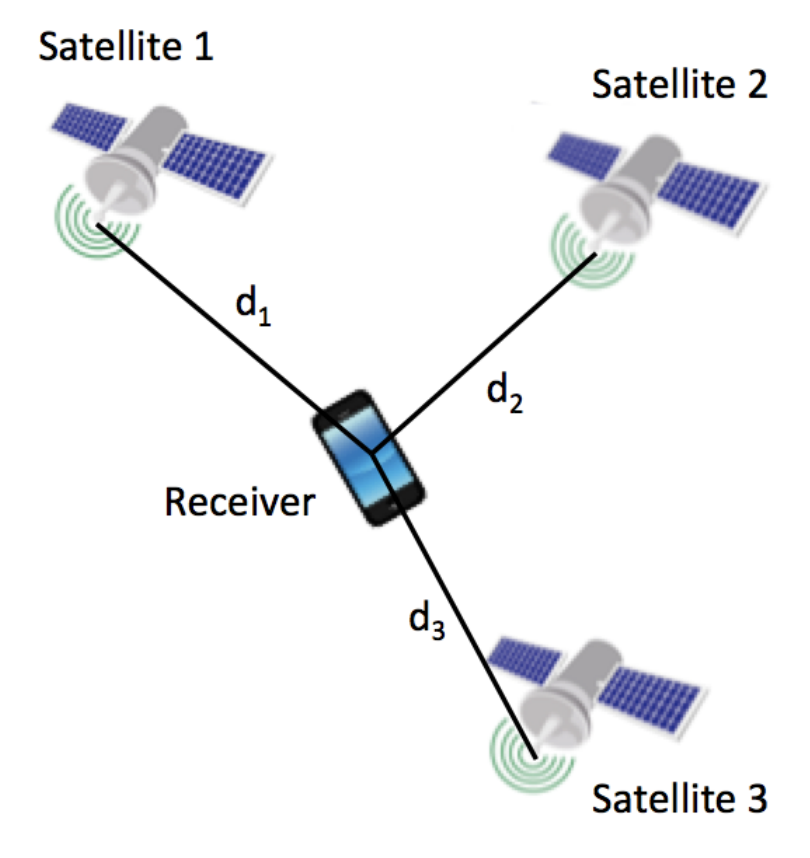
\includegraphics[scale=0.45]{../trilateration-1}
\end{figure}

\begin{enumerate}
    \item Based on the provided information above, which of the following variables are known? Which are unknown (the ones we are trying to solve for)?

        \begin{itemize}
            \item The position of each satellite $\vec{p}_i$
            \item Our current position $\vec{x}$
            \item The transmitted signals $\vec{s}_i^{(\tau_i)}$
            \item The distances from our current position to each satellite $d_i$
        \end{itemize}
    \answerbox{2cm}

    \item How can we express $d_i$ in terms of $\vec{p}_i$ and $\vec{x}$? How many such equations can we set up in total?

    \answerbox{5cm}


    \item Recall that an APS can help us determine where we are. Which variable given in the question corresponds to our current location?

    \answerbox{1cm}

    \item Based on the system of equations we set up in part 2, how can we solve for our current position?

    \answerbox{6cm}

    \item If our current position can be represented by an $n$-dimensional vector, how many satellites do we need to be able to solve for our position?

    \answerbox{1cm}

    \item As shown below geometrically, we can represent the area of coverage by each satellite as a circle with a radius of $d_i$. Explain why the radius of each circle is $d_i$, and how finding our current position is equivalent to finding the point of intersection among the circumferences of the circles.
    \begin{figure}[H]
        \centering
        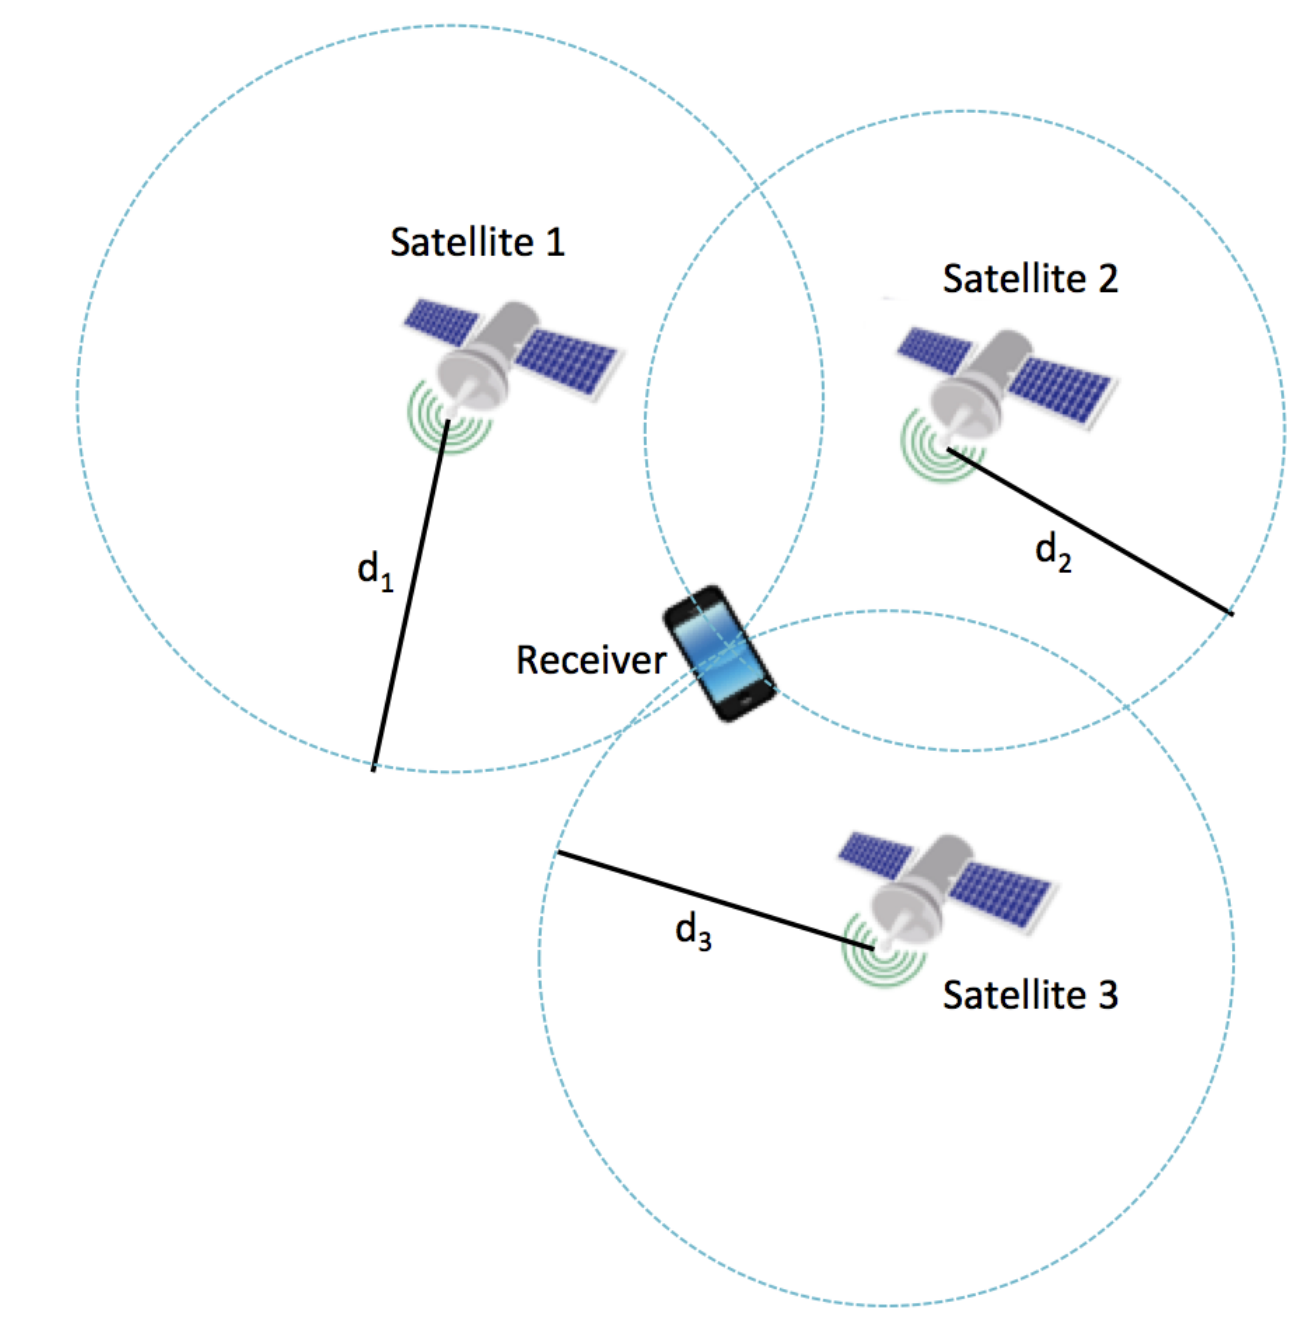
\includegraphics[scale=0.3]{../trilateration-2.png}
    \end{figure}

    \answerbox{4cm}

    \item Now that we have figured out where we are, it is time for us to decode the message! Recall that what our phone receives is a linear combination of these transmitted signals:
    $$\vec{r} = \alpha_1 \vec{s}_1^{(\tau_1)} + \alpha_2 \vec{s}_2^{(\tau_2)} + \hdots + \alpha_m \vec{s}_m^{(\tau_m)}$$
    From the expression above, which of the following variables are we trying to solve for?
    \begin{itemize}
        \item The scaling (attenuating) constant $\alpha_i$
        \item The original signal sent by the satellite $\vec{s}_i$
        \item The delay in the transmission of the signal $\tau_i$
    \end{itemize}

    \answerbox{3cm}

    \item To solve for the unknown variables from the previous part, we can use the \textbf{least squares} method. How can we reformulate the given expression and information above as a \textbf{least squares} problem? In other words, if we are to rewrite the problem in the form:
    $$A\vec{v} \approx \vec{b},$$
    what would $A$, $\vec{v}$, and $\vec{b}$ be equal to respectively?
    
    \answerbox{4cm}

    \item What is the solution using the \textbf{least squares} method?
    
    \answerbox{3cm}

    \item Does there exist a case where least squares would not work? Write down a sufficient condition where we have to resort to some other techniques to recover the original message.

    \answerbox{3cm}

    \item If we are to solve this problem using Orthogonal Matching Pursuit (OMP) instead of least squares, what is one assumption made by this technique?

    \answerbox{2cm}

    \item Describe what the stopping conditions for OMP are. In other words, how do we know when to stop running the OMP algorithm?

    \answerbox{2cm}

\end{enumerate}